\chapter{Introduction}

This article is a follow-up of the earlier article that I wrote as a part of a submission for the subject ESC612 (From wire to wireless), "\emph{Measurement of gravity by the voltage difference induced on a solenoid by a free-falling magnet.}" In that article, I approximated a solenoid as a simple circular loop that lies on the $x-y$ plane, and let the magnet hover at height $h$ over it. At the end, the gravitational acceleration measured was $9.52\unit{\meter\per\second}$, which is frankly better than I expected. However, I think that the $g$ value could be better if the geometry of the solenoid is actually used. Therefore, this article is going to address the magnetic flux of an actual solenoid, and compare it with the two other approximations that are commonly used.

\section{Geometries of the solenoid and its approximation}

\subsection{Geometry of an actual solenoid}

The solenoid is modeled as a helix that lies along the $z$ axis and centered at $(x, y) = (0, 0)$ shown in \cref{fig:actual-solenoid}
\begin{figure}[ht]
	\centering
	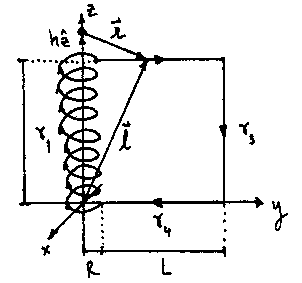
\includegraphics{solenoid.pdf}
	\caption{The solenoid's geometry}
	\label{fig:actual-solenoid}
\end{figure}

The solenoid of height $\frac{H}{2\cpi}$ that's wounded around itself $\omega$ times, where $\omega \in \mathbb{Z}$ is parameterized by the contour $\gamma$ which is given in four parts: $\gamma_1,\dots, \gamma_4$. $\gamma_1$ represents the actual solenoid, parameterized by
\begin{align}
	 & \gamma_1: \ab(x = R\sin(\omega\alpha), y = R\cos(\omega\alpha), z = \frac{H}{2\cpi}) & \alpha \in [0, 2\cpi]
\end{align}
The contour $\gamma_2$ to $\gamma_4$ represents the wire that connects the bottom of the solenoid to the top:
\begin{align}
	 & \gamma_2: \ab(x = 0, y = L\alpha + R, z = H)  & \alpha \in [0, 1] \\
	 & \gamma_3: \ab(x = 0, y = L + R, z = \alpha H) & \alpha \in [1, 0] \\
	 & \gamma_4: \ab(x = 0, y = L\alpha + R, z = 0)  & \alpha \in [1, 0]
\end{align}

\subsection{Geometry of the approximations}

Before I wrote this article, I decided asked my good friend, \emph{Nattawee Wiwatthanakul} for an opinion on how the magnetic flux may be calculated. He proposed that the solenoid's flux can be approximated with a stack of circular wires shown in \cref{fig:stacked-circles}. The wire also has radius $R$, and is stacked on itself $\omega$ times ($\omega \in \mathbb{Z}^+$), reaching the height of $H$.

\begin{figure}[ht]
	\centering
	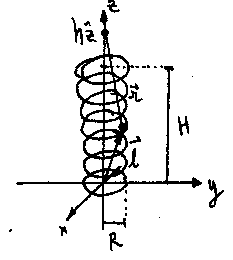
\includegraphics{stackedcircles.pdf}
	\caption{Stacked circles approximation for the solenoid}
	\label{fig:stacked-circles}
\end{figure}

Each loop contributes its own magnetic flux ${\mflux}_i$, and thus the total magnetic flux must be the sum of each loop:
\begin{equation}
	\mflux = \sum_{i = 0}^{\omega}{\mflux}_i
\end{equation}

\section{Magnetic flux}

The magnetic flux, $\mflux$ is given by
\begin{equation}
	\mflux = \sint\vv{B}\cdot\odif{\vv{a}} \label{eq:faradays-law-line-integral}
\end{equation}
where $\vv{B}$ is the magnetic field that's on the wire, and $\odif{\vv{a}}$, the area integration element. However, this cannot be done with the geometry of the solenoid because the area enclosed by the wire cannot be parameterized in a simple way. Thus, the area integral must be transformed into a line integral using the Green's theorem. Given that the vector magnetic potential $\vv{A}$ where $\vv{B} = \curl\vv{A}$, \cref{eq:faradays-law-line-integral} becomes
\begin{equation}
	\mflux = \sint\ab(\curl\vv{A})\cdot\odif{\vv{a}} = \oint_{\gamma}\vv{A}\cdot\odif{\vv{l}}.
\end{equation}
By parameterization,
\begin{equation}
	\oint_{\gamma}\vv{A}\cdot\odif{\vv{l}} = \oint\vv{A}\cdot\odv{\vv{l}}{\alpha}\odif{\alpha}
\end{equation}
